\documentclass[english]{scrartcl}
\usepackage[T1]{fontenc}
\usepackage[utf8]{inputenc}
\usepackage[scaled=.8]{beramono}
\usepackage{geometry}
\geometry{verbose,tmargin=3cm,bmargin=3cm,lmargin=3cm,rmargin=3cm}
\usepackage{microtype}
\usepackage[parfill]{parskip}
\usepackage{amsmath}
\usepackage{graphicx}
\usepackage{hyperref}
\usepackage{nameref}
\usepackage{float}
\usepackage{listings}
\usepackage{color}
\usepackage{fancyhdr}
\usepackage{blindtext}
\usepackage[noend]{algpseudocode}
\usepackage{algorithm}
\algnewcommand{\LineComment}[1]{\State \(\triangleright\) #1}

\usepackage{subcaption}
\usepackage{booktabs}
\usepackage[htt]{hyphenat}

\pagestyle{fancy}
\fancyhf{}
\rhead{Group 2}
\lhead{DM: Correlation Clustering}
\cfoot{\thepage}

\newcommand*{\fullref}[1]{\hyperref[{#1}]{\autoref*{#1}~\nameref*{#1}}}

\definecolor{darkgray}{rgb}{0.66, 0.66, 0.66}
\definecolor{asparagus}{rgb}{0.53, 0.66, 0.42}

\lstdefinestyle{s}{
  commentstyle=\color{darkgray},
  keywordstyle=\bfseries,
  morekeywords={},
  stringstyle=\color{asparagus},
  basicstyle=\ttfamily\footnotesize,
  breakatwhitespace=false,
  keepspaces=true,
  numbersep=5pt,
  showspaces=false,
  showstringspaces=false,
}

\lstset{style=s}

\begin{document}

\title{Data Mining\\Programming Assignment 1: Correlation Clustering}

\author{Sonja Biedermann \and Thilo Hannes Fryen \and Chan Dat Dennis Huyen \and David Turner}

\maketitle
\tableofcontents

\section{ORCLUS}

We decided to implement the ORCLUS algorithm. ORCLUS is a spin on $k$-means
which utilizes eigensystems to adapt the distance measure to non axis parallel
correlation clusters.

We picked this algorithm because the paper is easy to read and contains good
pseudo code which is of utmost importance when trying to actually implement
the described algorithm.

Furthermore, since $k$-means was the first clustering algorithm we studied, it will forever
have a special Gaussian-shaped spot in our heart---which makes ORCLUS, as a
spiritual successor, a natural choice.

\subsection{Description}

The algorithm proceeds in rounds in which the dimensionality of the clusters
and the number of clusters is gradually reduced. The rate at which this happens should
not be too quickly, to which end the authors propose two parameters $\alpha$ and $\beta$
and a relation between these two, by which one can be calculated from the other. They
suggest an $\alpha$ of 0.5, which we've also adopted.

In each round, the algorithm undertakes an assignment step which is the same as
in $k$-means. Every point is assigned to the closest centroid. However, as a
next step, the eigenvectors associated with the smallest spread are computed on
a per cluster basis---the rationale behind this is that those vectors define a
subspace in which the points cluster well, i.e. have a low contribution to the
overall cluster energy. The cardinality of this vector set dictates the dimensionality
of the subspace to which the points are projected. The points are then projected
into the subspace defined by these vectors, which modifies their distances to
each other.

To reduce the amounts of clusters---the algorithm starts with more seeds than
requested by the user, we've chosen to start with 5 times as many as the
authors offer no suggestions---a merging step is performed next. Although quite
lengthy, this operation is pretty simple. The objective is to find pairs of
clusters which can be merged such that the overall cluster energy stays low.
For this, all pairs of clusters are examined, their centroid and energy
computed and then the cluster-pairs with the lowest energy are picked to be merged, being
careful to update all relevant data structures after each merge.

These three steps are repeated until the desired dimensionality and number of
clusters are reached. After a final assignment step the clustering is returned.

\subsection{Pseudocode}

The core algorithm is defined in Algorithm~\ref{alg:main}. Algorithms~\ref{alg:ass},~\ref{alg:find}~and~\ref{alg:merge}
cover the assignment, subspace determination, and merging of clusters.

%%%%%%%%%% ORCLUS
\begin{algorithm}
\begin{algorithmic}
\Function{orclus}{\textit{Database: $DB$, \# of Clusters: $k$, \# of Dimensions: $l$}}
    \LineComment{$C_i \Rightarrow$ current cluster $i$}
    \LineComment{$\varepsilon_i \Rightarrow$ set of vectors defining subspace for cluster $C_i$}
    \LineComment{$k_c \Rightarrow$ current \# of seeds}
    \LineComment{$l_c \Rightarrow$ current dimensionality}
    \LineComment{$S = \{s_1, s_2, ... s_{k_c}\} \Rightarrow$ current set of seeds}
    \State $k_c = k_0;$ $l_c = d;$ \Comment{$k_0 \Rightarrow$ initial \# of seeds} \Comment{$d \Rightarrow$ dimension of the data}
    \State Pick $k_0 > k$ points from $DB$ an denote by $S$;
    \Comment{e.g. randomly or K-means++}
    \ForAll{$i \in \{1 ... k_c\}$}
        $\varepsilon_i = D$; \Comment{initially, $\varepsilon_i$ is the original axis-system}
    \EndFor
    \State $\alpha = 0.5;$ $\beta = e^{-\log (l_c/l)\log (1/\alpha) / \log (k_c/k)};$
    \While{$k_c > k$}
        \LineComment{partition the database by assigning each object to its closest seed}
        \State $s_1 ... s_{k_c},$ $C_1...C_{k_c} =$ \Call{assign}{$DB$, $S$, $\varepsilon$};
        \LineComment{determine current subspace associated with each cluster}
        \ForAll{$i \in \{1...k_c\}$}
            $\varepsilon_i =$ \Call{findVectors}{$C_i$, $l_c$};
        \EndFor
        \LineComment{reduce number of seeds and dimensionality associated with each seed}
        \State $k_{new} =$ \Call{max}{$k$, $k_c * \alpha$}; $l_{new} =$ \Call{max}{$l$, $l_c * \beta$};
        \State $s_1...s_{k_{new}},$ $C_1...C_{k_{new}},$ $\varepsilon_1...\varepsilon_{k_{new}} =$ \Call{merge}{$C_1...C_{k_c}$, $k_{new}$, $l_{new}$};
        \State $k_c = k_{new};$ $l_c = l_{new};$
    \EndWhile
    \State $s_1...s_{k_c},$ $C_1...C_{k_c} =$ \Call{assign}{$DB$, $S$, $\varepsilon$};
    \State \Return $(C_1...C_{k_c})$;
\EndFunction
\end{algorithmic}
\caption{ORCLUS}
\label{alg:main}
\end{algorithm}

%%%%%%%%%% ASSIGN
\begin{algorithm}
\begin{algorithmic}
\Function{assign}{$DB$, $s_1...s_{k_c}$, $\varepsilon_1...\varepsilon_{k_c}$}
   \ForAll{$i \in \{1...k_c\}$}
        $C_i = \emptyset$;
   \EndFor
   \ForAll{$p \in DB$}
       \LineComment{distance of point $p$ to $s_i$ in subspace $\varepsilon_i$}
        \ForAll{$i \in \{1...k_c\}$}
            \Call{pdist}{$p$, $s_i$, $\varepsilon_i$};
        \EndFor
        Determine the seed $s_i$ with the least value of \Call{pdist}{$p$, $s_i$, $\varepsilon_i$} and add $p$ to $C_i$;
   \EndFor
   \ForAll{$i \in \{1 ... k_c\}$}
        $s_i =$ \Call{$\bar{X}$}{$C_i$};
        \Comment{set $s_i$ to new cluster center}
   \EndFor
   \Return $(s_1...s_{k_c},$ $C_1...C_{k_c})$
\EndFunction
\end{algorithmic}
\caption{Assignment step}
\label{alg:ass}
\end{algorithm}

%%%%%%%%%% FINDVECTORS
\begin{algorithm}
\begin{algorithmic}
\Function{findVectors}{\textit{Cluster of Points: $C$, Dimensionality of Projection: $q$}}
    \State Determine the $d*d$ covariance matrix $M$ for $C$;
    \State Determine the eigenvectors of matrix $M$;
    \State $\varepsilon =$ Set of eigenvectors corresponding  to smallest $q$ eigenvalues;
    \State \Return $(\varepsilon)$
\EndFunction
\end{algorithmic}
\caption{Procedure for determining cluster subspaces}
\label{alg:find}
\end{algorithm}

%%%%%%%%%% MERGE
\begin{algorithm}
\begin{algorithmic}
\Function{merge}{$C_1...C_{k_c}$, $k_{new}$, $l_{new}$}
    \ForAll{$i,j \in \{1...k_c\}, i < j$}
        \LineComment{define $\varepsilon'_{ij}$ by eigenvectors for $l_{new}$ smallest eigenvalues}
        \State $\varepsilon'_{ij} =$ \Call{findVectors}{$C_i \cup C_j$, $l_{new}$};
        \State $s'_{ij} =$ \Call{$\bar{X}$}{$C_i \cup C_j$};
        \Comment{Centroid of $C_i \cup C_j$}
        \LineComment{compute projected energy of $C_i \cup C_j$ in subspace $\varepsilon'_{ij}$}
        \State $r_{ij} =$ \Call{clusterEnergy}{$C_i \cup C_j$, $\varepsilon'_{ij}$};
    \EndFor
    \While{$k_c > k_{new}$}
        \ForAll{$i,j \in \{1...k_c\}, i < j$}
            Find smallest value of $r_{i'j'}$;
        \EndFor
        \LineComment{merge the corresponding clusters $C_{i'}$ and $C_{j'}$}
        \State $s_{i'} = s'_{i'j'}$; $C_{i'} = C_{i'} \cup C_{j'}$; $\varepsilon_{i'} = \varepsilon'_{i'j'}$;
        \State Discard $s_{j'}$ and $C_{j'}$;
        \State Renumber the seeds/clusters indexed larger than $j'$ by subtracting 1;
        \ForAll{$i,j \geq j'$}
            Renumber the values of $s'_{ij}$, $\varepsilon_{ij}$, $r_{ij}$ correspondingly;
        \EndFor
        \LineComment{recompute $r_{i'j}$ pairwise for new cluster $i'$}
        \ForAll{$j \neq i' \in \{1...k_c - 1\}$}
            \State $\varepsilon'_{i'j} =$ \Call{findVectors}{$C_{i'} \cup C_j$, $l_{new}$};
            \State $s'_{i'j} =$ \Call{$\bar{X}$}{$C_{i'} \cup C_j$};
            \State $r_{i'j} =$ \Call{clusterEnergy}{$C_{i'} \cup C_j$, $\varepsilon'_{i'j}$};
        \EndFor
        $k_c = k_c - 1$;
    \EndWhile
    \Return $(s_1...s_{k_{new}}$, $C_1...C_{k_{new}}$, $\varepsilon_1...\varepsilon_{k_{new}})$
\EndFunction
\end{algorithmic}
\caption{Procedure for merging clusters}
\label{alg:merge}
\end{algorithm}

\subsection{Implementation}

We chose to implement the algorithm in Python 3. The implementation is rather straight
forward and only depends on NumPy and some functionality from Python's standard
library.

Notably we use \texttt{numpy.linalg.eigh} to decompose the cluster matrices
into eigenvalues and eigenvectors. We know PCA could also be used but online
literature\footnote{\url{https://stackoverflow.com/questions/50358310/how-does-numpy-linalg-eigh-vs-numpy-linalg-svd}}
suggests that the LAPACK routines utilized in NumPy's implementation of
\texttt{eigh} perform a tiny sliver better than SVD, which we expect to be used
in \texttt{sklearn.decomposition.PCA}.  However, this probably would make no
practical difference whatsoever.

The initial seeds are distributed using the kmeans\texttt{++} initialization strategy,
although we have also implemented a completely random initialization strategy.
If the initial seed count is chosen to be high enough, this strategy actually
seems to be beneficial, as it returns good partitions and is also faster. Thus
we also included a random seed picking startegy, although we didn't use it
during the evaluation.

\pagebreak
\section{Evaluation}

We will be comparing ourselves to the ELKI implementation on 4 synthetic datasets
using the NMI as scoring method. The datasets were generated using ELKI's data generator.
We used flat Gaussian distributions as correlation clusters and added noise points
to disturb the algorithm.

\subsection{Methodology}

The evaluation should be fully reproducible. File \texttt{eval.sh} contains the calls made to our
test scripts and ELKI. \texttt{summary.rb} is a Ruby script which processes the results, outputs
an overview table and also generates a \texttt{gnuplot}-ready plot file for plotting a boxplot of
the results.

The scripts \texttt{show\_data.py} can be used to view the datasets contained in \texttt{data/},
\texttt{elki\_results\_to\_csv.py} consolidates the output of ELKI into one single \texttt{.csv}
file which can be plotted and compared to our results using the \texttt{plot\_results.py} script.

We execute the test runs 5 times and note their resulting NMIs as well as the clusterings with the
best NMI score. We average using the arithmetic mean.

\subsection{Simple dataset}

As a simple first dataset we generate a 2-dimensional data set containing 3 clusters that are very clearly
separated, one of which is a bit fatter than the stereotypical correlation cluster, and which is
axis-parallel. Figure~\ref{fig:test} shows the results obtained by our implementation
and the result obtained by the implementation contained in ELKI. They are identical---notably misclassifying one
single point which would belong to the fat axis-parallel cluster.

\begin{figure}[tb]
    \centering
    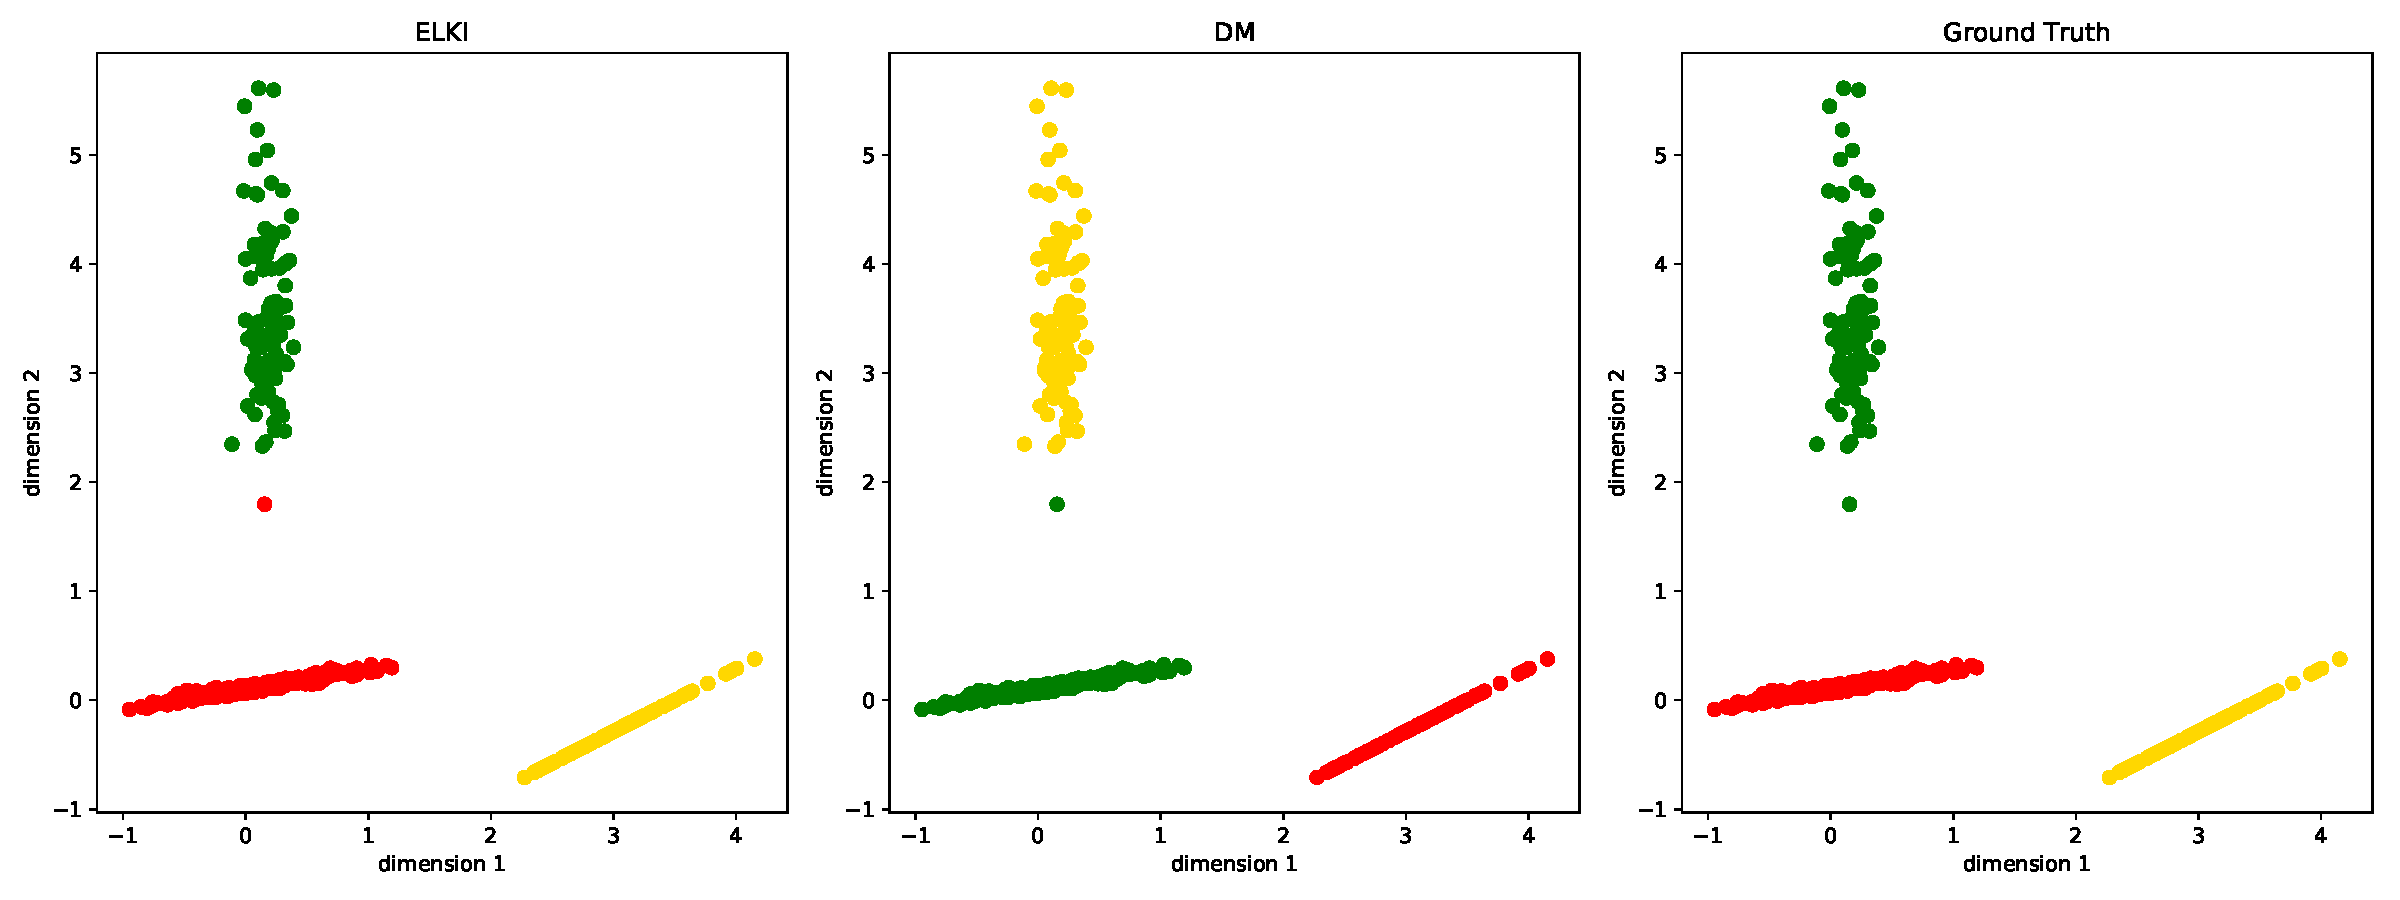
\includegraphics[width=\textwidth]{img/test_cmp}
    \caption{Results on the \texttt{test} dataset}
    \label{fig:test}
\end{figure}

\subsection{Simple dataset with added noise}

We want to torment ORCLUS by adding noise to the previous trivial dataset.
It should perform much worse, since ORCLUS has no notion of noise by default
(and, although the authors recommend a simple scheme for implementing outlier
detection, this does not seem to be implemented in ELKI), but it is interesting
to see how the two implementation compare on a problematic dataset.

Figure~\ref{fig:noisy-cmp} show the results
of our implementation and ELKI's implementation as well as the ground truth.

\begin{figure}[tb]
    \centering
    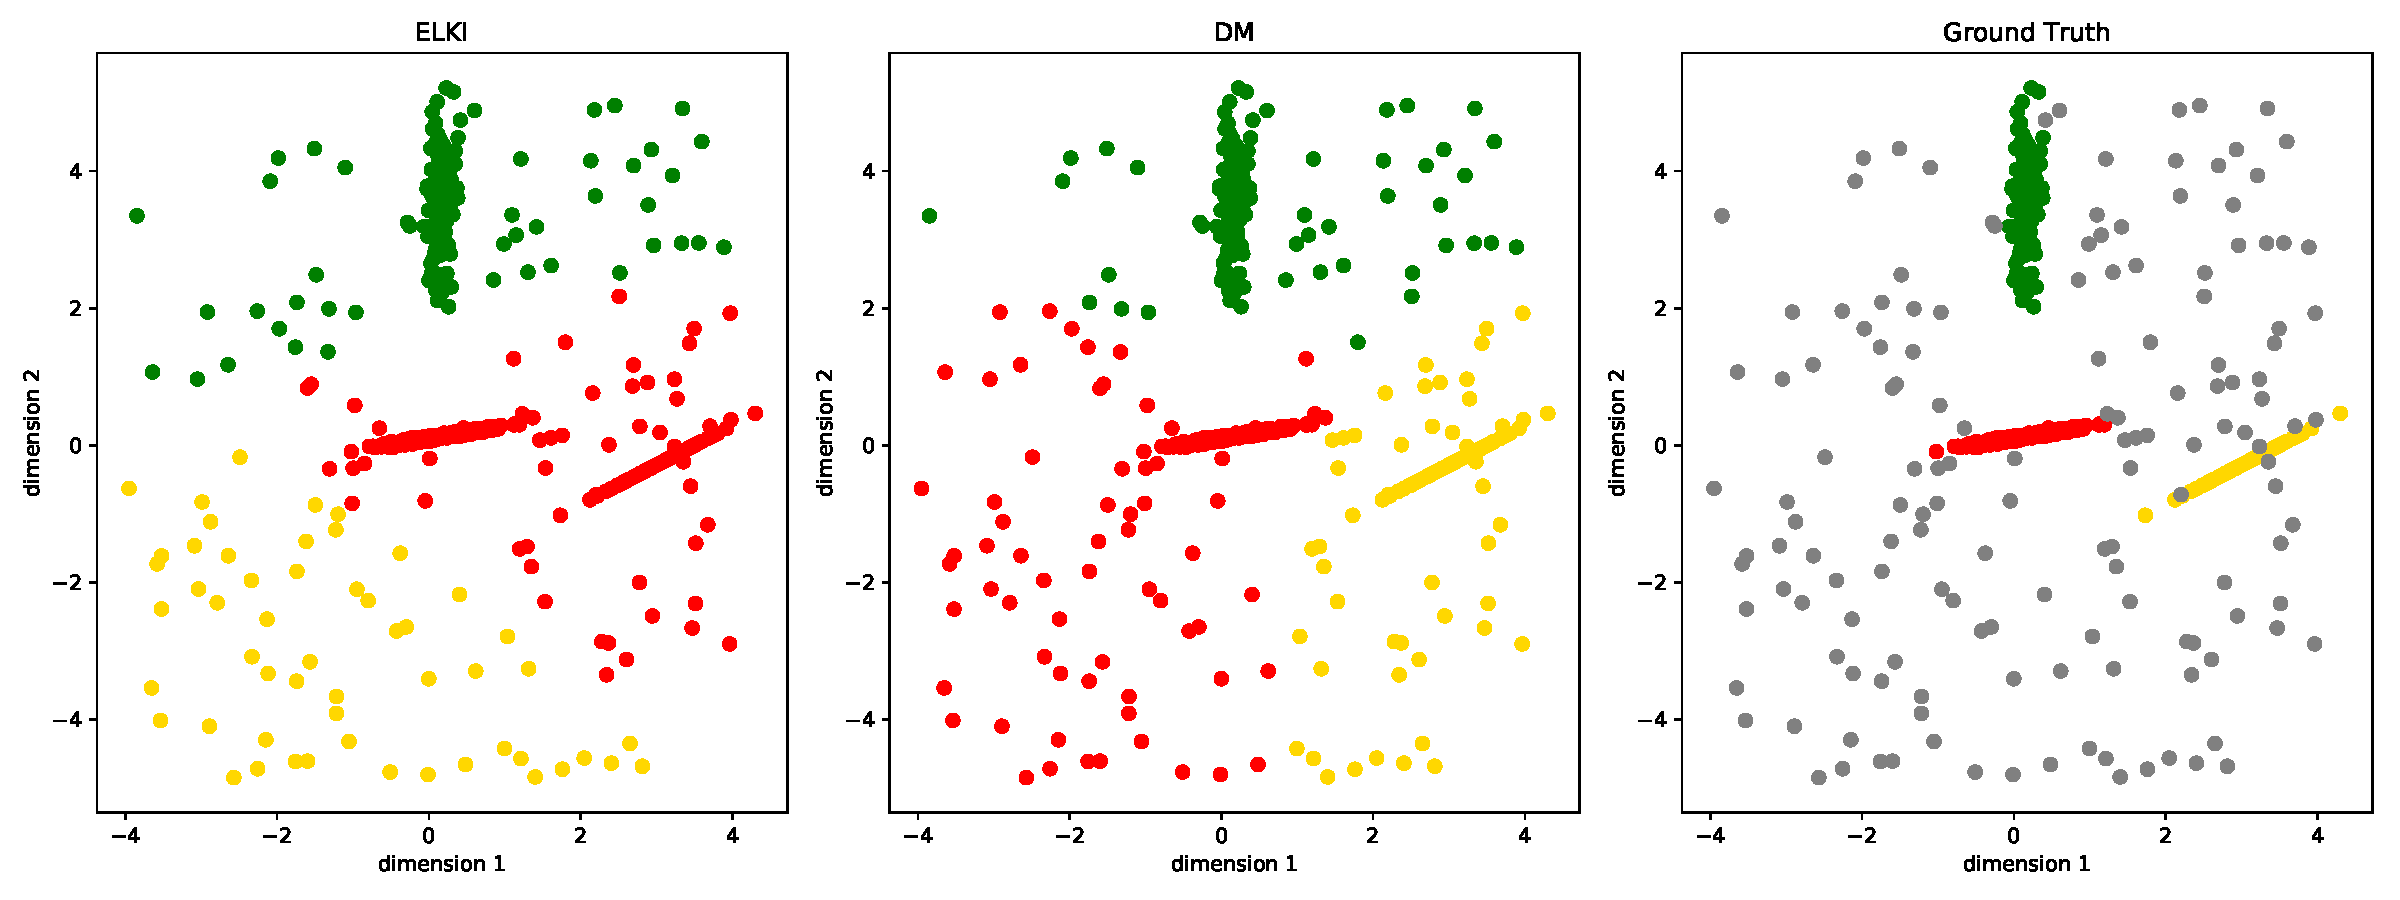
\includegraphics[width=\textwidth]{img/test_noisy_cmp}
    \caption{Results for dataset \texttt{test\_noisy}}
    \label{fig:noisy-cmp}
\end{figure}

\subsection{Clusters that are noise in some subspaces}

It seems like a common situation in real-world data that clusters are present
in some subspaces, but are very dispersed in other subspaces, where other
clusters may reside---thus clusters in some subspaces are noise in others. We
would thus expect the algorithm to struggle. Figure~\ref{fig:true_higher_dim} depicts
the ground truth for this data set.

Figure~\ref{fig:higher_dim_res} shows the results for both implementations.
Interestingly, our implementation manages to obtain clusterings that
look tidier. However, the NMIs are pretty close, as the tidiness of
the clustering does not match the actual structure in the data.

Note that we used more intial seeds for this dataset, as this seems to
help a lot here.

\begin{figure}[p]
    \centering
    \begin{subfigure}{0.6\textwidth}
        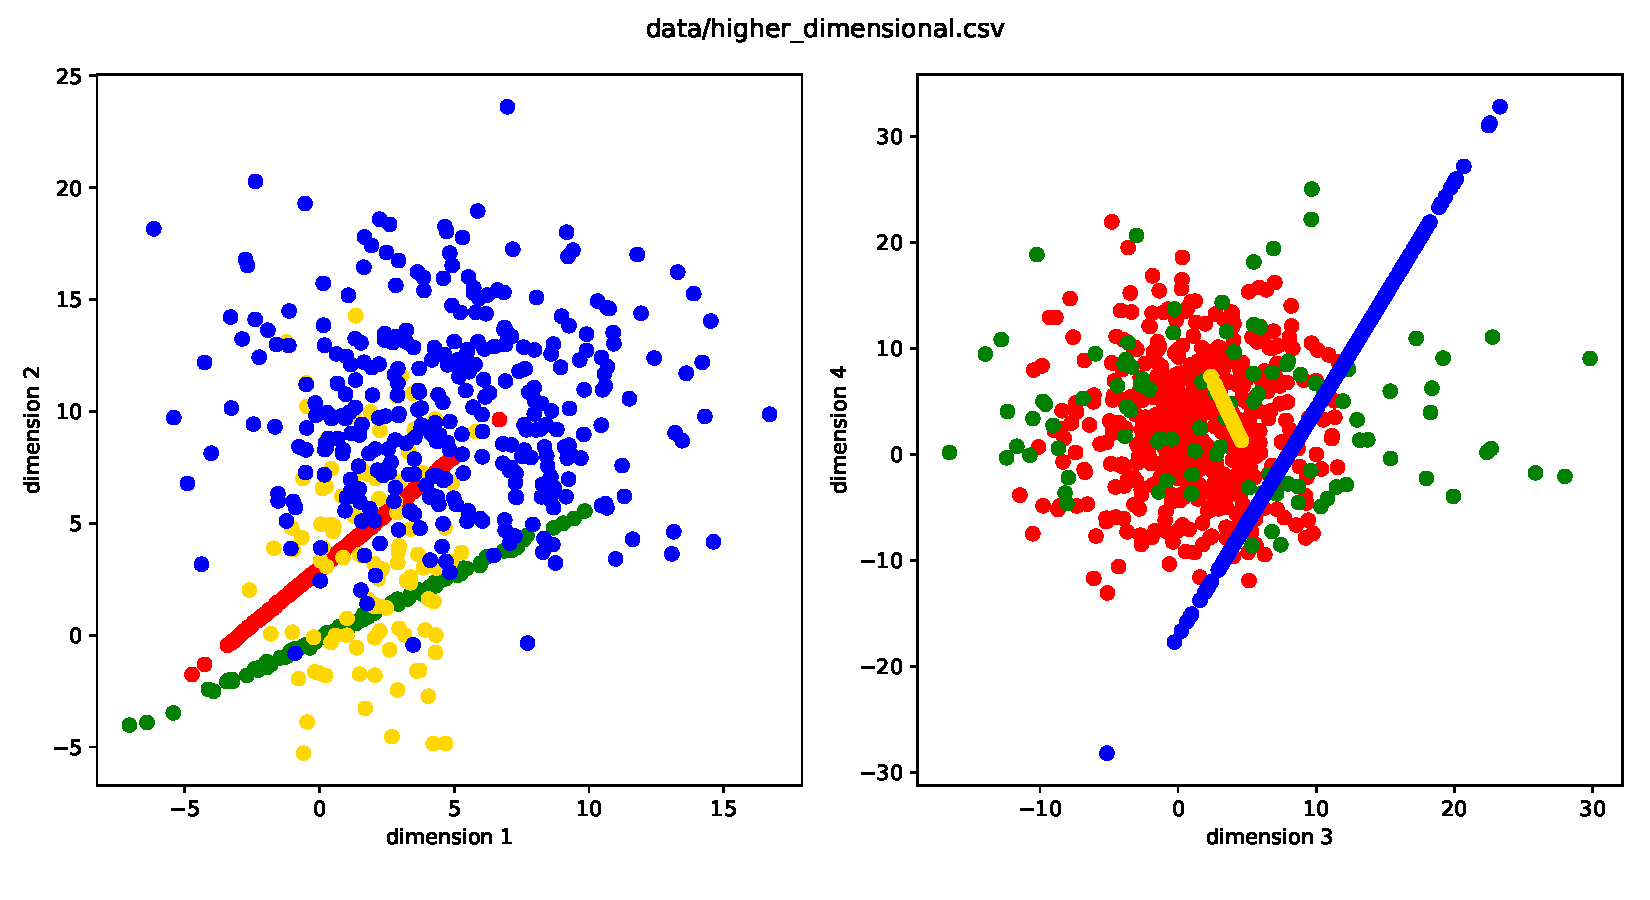
\includegraphics[width=\textwidth]{img/higher_dimensional}
        \caption{Ground truth for \texttt{higher\_dimensional}}
        \label{fig:true_higher_dim}
    \end{subfigure}%
    \\
    \begin{subfigure}{0.6\textwidth}
        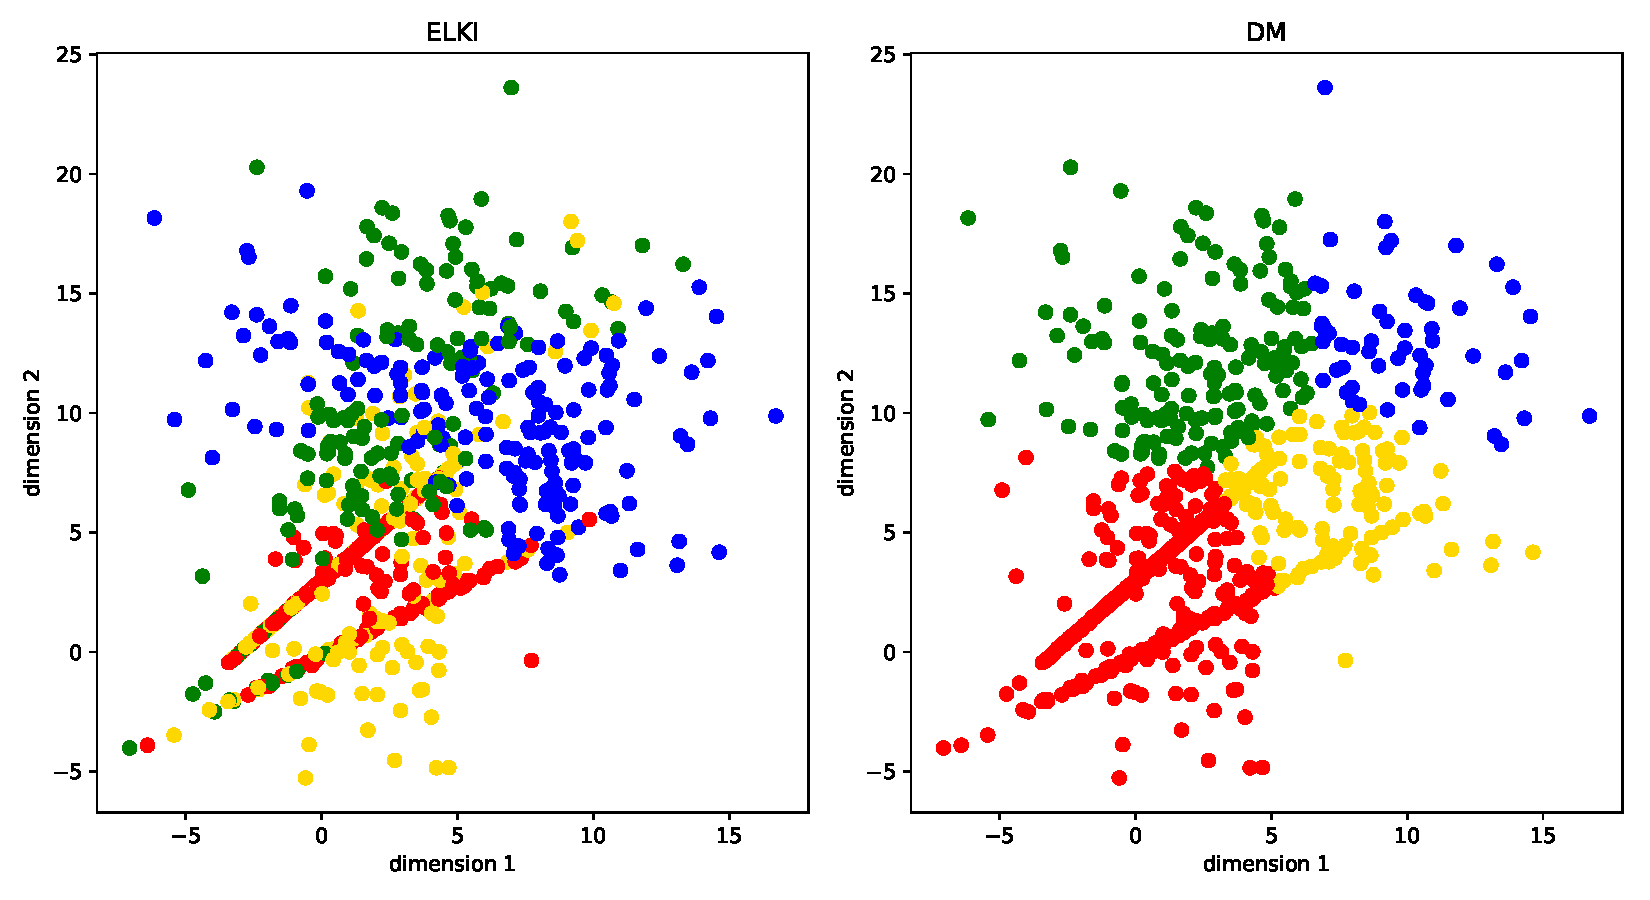
\includegraphics[width=\textwidth]{img/higher_dimensional_cmp}
        \caption{Results of ELKI vs. our implementation}
        \label{fig:higher_dim_res}
    \end{subfigure}%
    \\
    \begin{subfigure}{0.6\textwidth}
        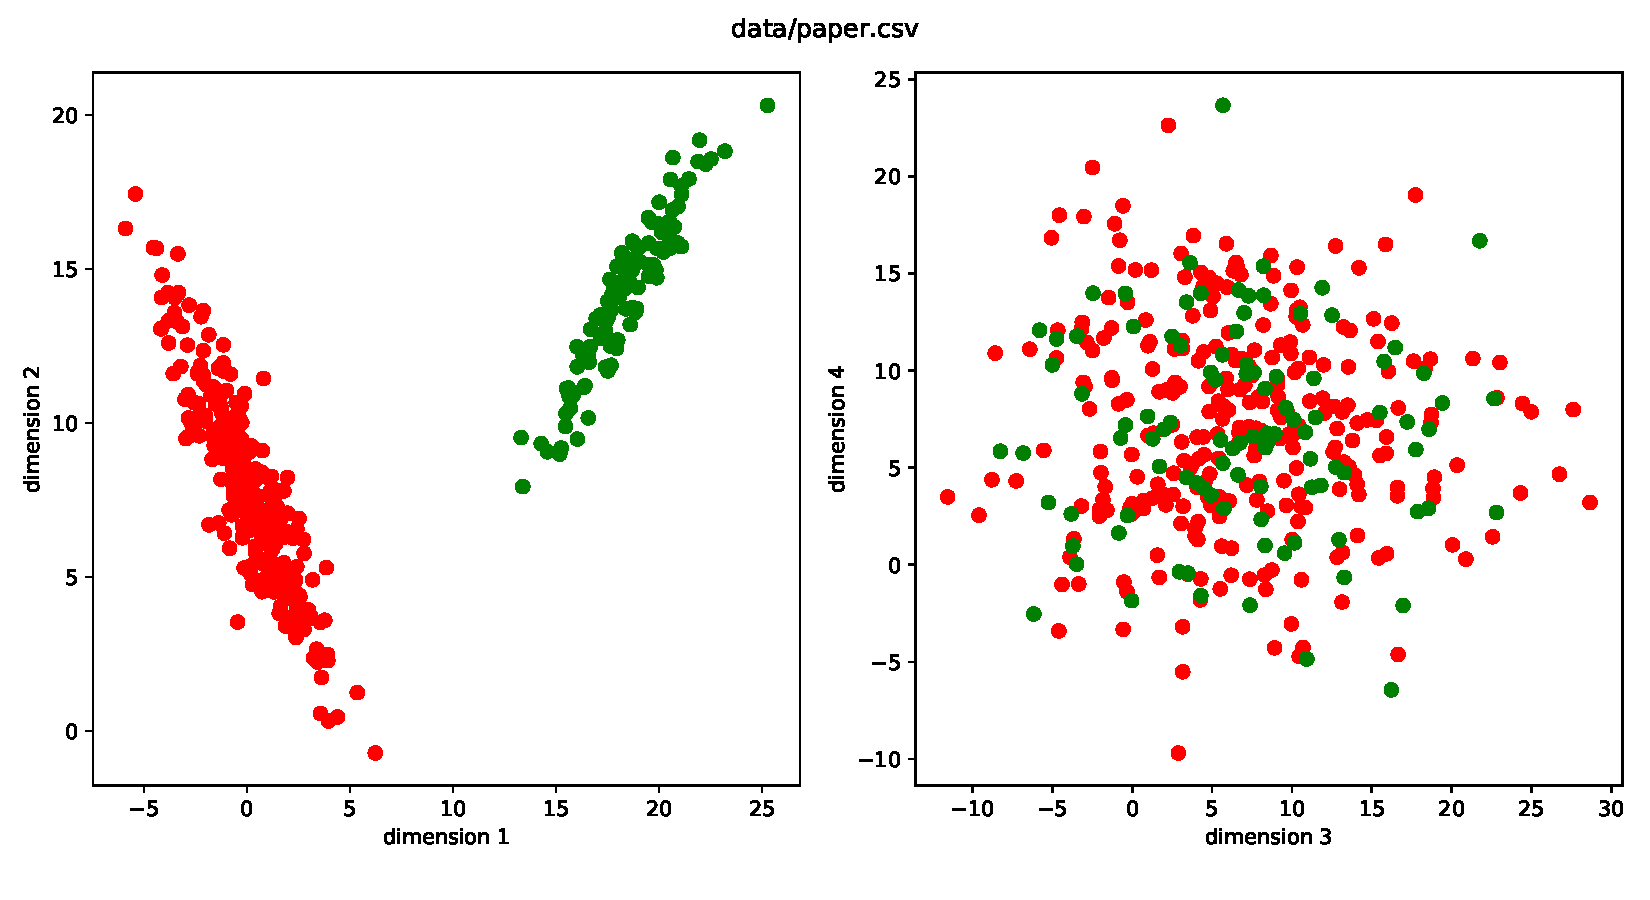
\includegraphics[width=\textwidth]{img/paper}
        \caption{Ground truth for \texttt{paper}}
        \label{fig:true_paper}
    \end{subfigure}%
    \\
    \begin{subfigure}{0.6\textwidth}
        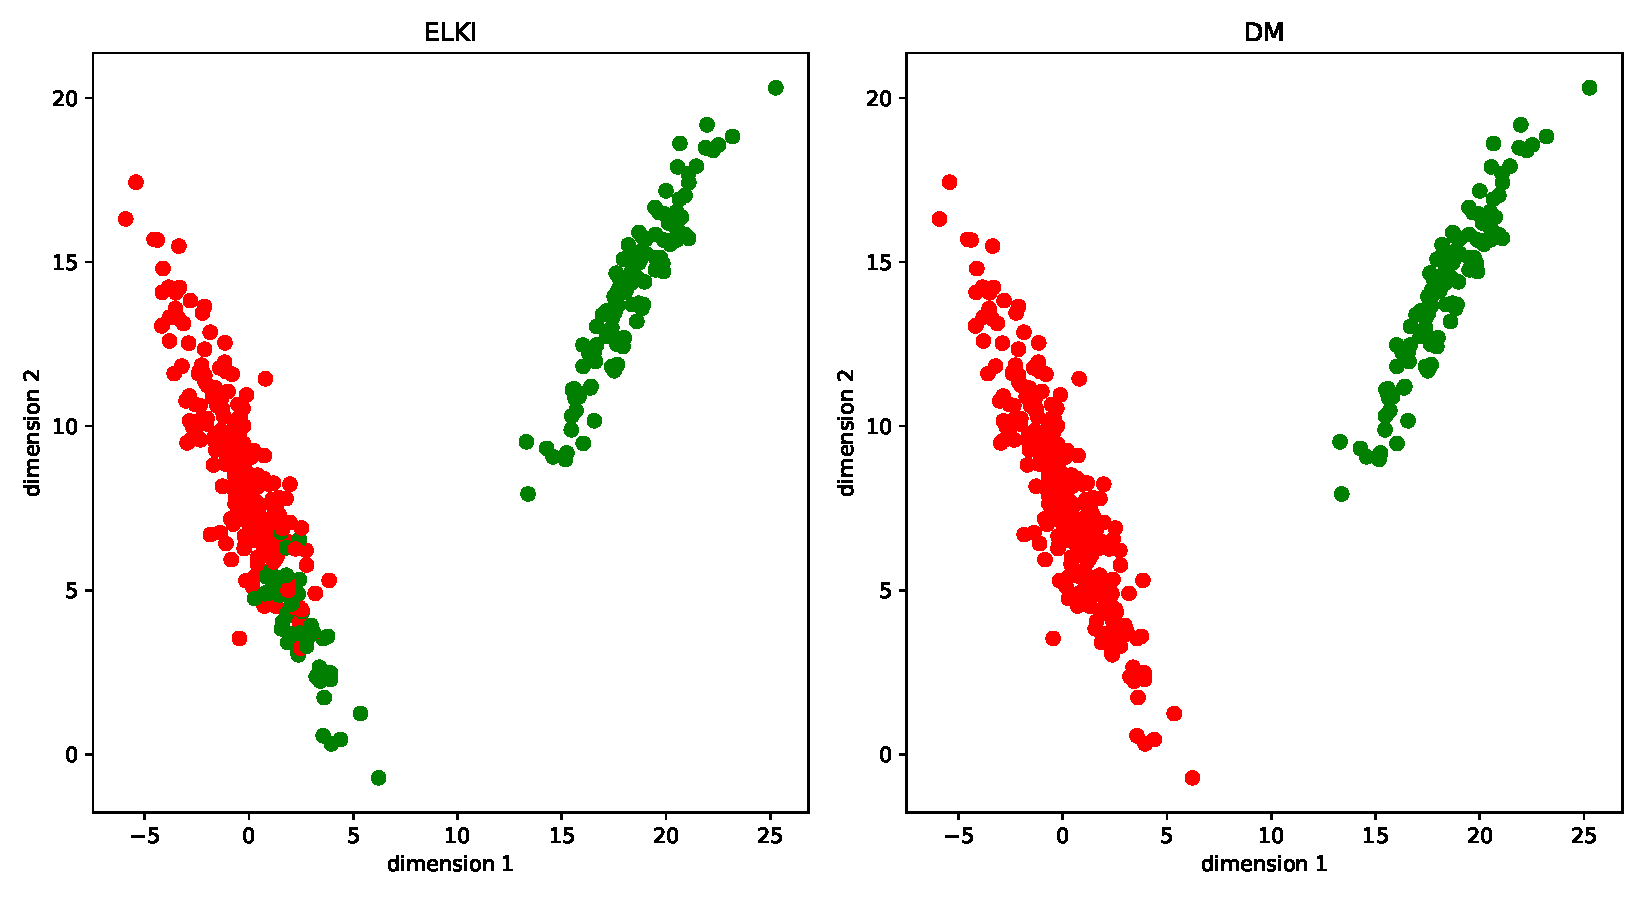
\includegraphics[width=\textwidth]{img/paper_cmp}
        \caption{Results of ELKI vs. our implementation}
        \label{fig:paper_results}
    \end{subfigure}
    \caption{Results on the \texttt{higher\_dimensional} and \texttt{paper} datasets compared to their ground truth}
\end{figure}

\subsection{Clusters with different rotations in some subspaces}

The final dataset is somewhat based on the example of projected clusters
in the paper. This dataset has two rotated clusters in the first two dimensions,
and Gaussian noise in the last two dimensions. We expect the algorithm to
correctly focus on the leading two dimensions and discard the other two.
Figure~\ref{fig:true_paper} shows this data set with the correct labels.

Note that this data set has an axis-parallel representation when picking the
first and third dimension (i.e. a noise dimension). This subspace seems to be
preferred by ELKI's implementation, as misclassified points are often at the
border of the correct cluster in this subspace. It could be that these outliers
(that are somehow assigned to the wrong cluster, e.g. by badly placed seeds)
destroy the PCA result, causing the algorithm to fall into a local minimum it
cannot escape from.

Figure~\ref{fig:paper_results} shows the results. As this is a very simple
data set, we are a bit worried that ELKI does not manage to find this
clustering in every try---out of 5 runs, only one run managed to reach a
NMI of 1. One run was even only able to reach a NMI of 0.005, which is
catastrophically small. Our implementation also returns wildly different
clusterings, which is unfortunate, as this dataset indeed does have
very clear clusters. The culprit is probably the noise dimensions
being considered, which will return rather unpredictable cluster basis
vectors.

\subsection{Summary}

Table~\ref{tab:overview} shows the results of our evaluation. The minimum,
maximum and average over the 5 runs are shown split between our implementation
(DM) and the implementation available in ELKI. Averages that are better than
ELKI's average NMI are written in bold, although note that some of the differences
are rather slight. Equal results are written in italic.

\begin{table}[]\centering
    \begin{tabular}{lrrrcrrr}\toprule
     & \multicolumn{3}{c}{DM} & \phantom{abc} & \multicolumn{3}{c}{ELKI}\\
    dataset & min & max & avg & & min & max & avg\\ \midrule
    test & 0.9869 & 0.9869 & \emph{0.9869} & & 0.9869 & 0.9869 & 0.9869\\
    test noisy & 0.539 & 0.6596 & \textbf{0.6352} & & 0.5372 & 0.6585 & 0.6342\\
    higher dimensional & 0.1892 & 0.3368 & \textbf{0.2631} & & 0.1881 & 0.3561 & 0.2578\\
    paper & 0.6466 & 1.0 & \textbf{0.8863} & & 0.0046 & 1.0 & 0.5594\\
  \bottomrule
  \end{tabular}
  \caption{Overview over NMI scores}
  \label{tab:overview}
\end{table}


\begin{figure}[t!]
    \centering
    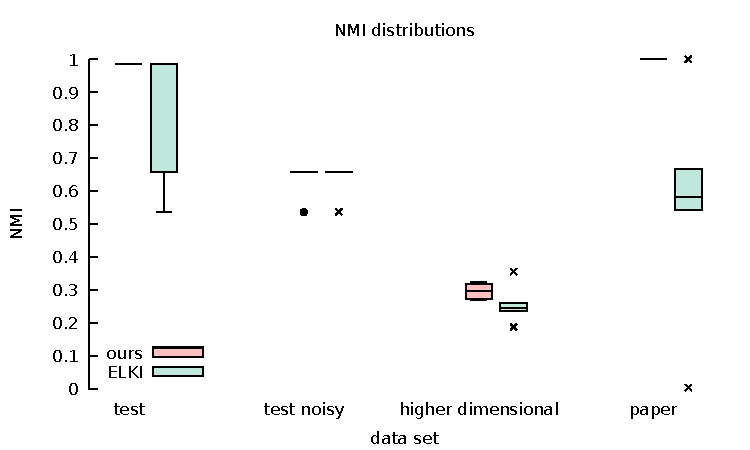
\includegraphics[width=\textwidth]{img/boxplt}
    \caption{Boxplot illustrating stability}
    \label{fig:box}
\end{figure}

Interestingly, our implementation appears to have a slight advantage over
ELKI's.  Notice especially the discrepancy with dataset \texttt{paper}, where
ELKI's implementation appears extremely unstable, while ours uncovers the
cluster structure perfectly 3 out of 5 times, with the two other results being of fairly similar quality. The biggest difference in our
implementation is that we use a different initialization strategy, namely
kmeans\texttt{++}---this might result in our algorithm having an easier time
converging to a good minimum since the cluster centers are already
well-separated. However, our implementation performed better even when using a
random seed picking strategy---we suspect that perhaps the eigenvalue
decomposition is implemented differently, or we are just lucky. We also want to
note that we use fewer initial seeds than ELKI, which defaults to $30 \cdot k$.

Figure~\ref{fig:box} shows a boxplot of the obtained NMI scores. A more stable implementation
would have a shorter box, i.e. less variance in the results. Our implementation appears
a bit more stable on the given datasets.

\end{document}
